\section{示例}

\subsection{图片}

如图\ref{F1}所示

\begin{figure}[H]
	\centering
	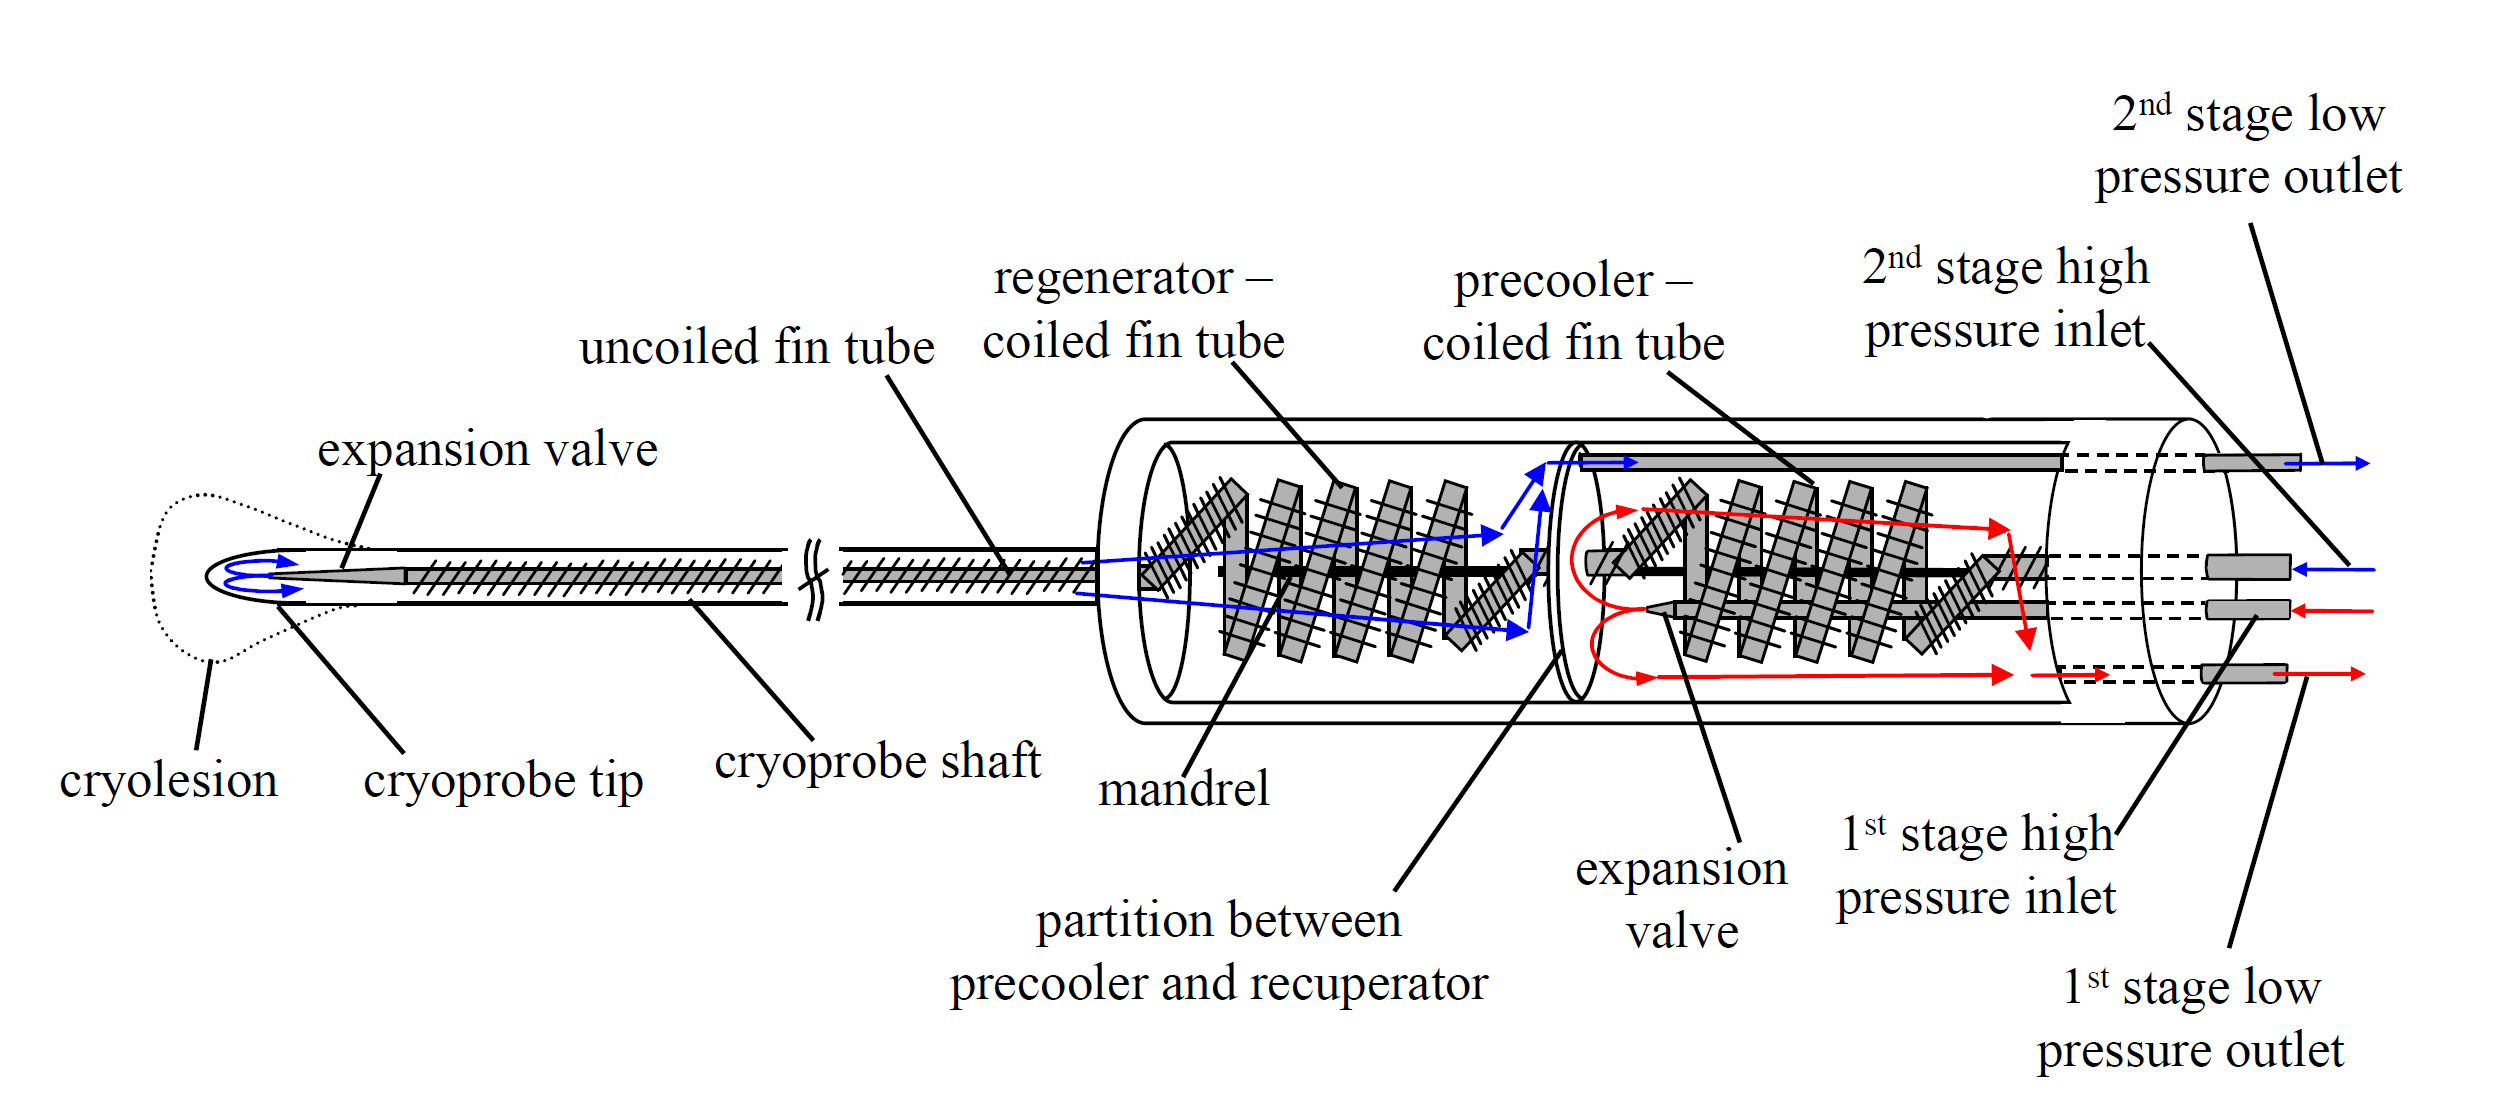
\includegraphics[width=\linewidth]{pics/1}
	\caption{封面示例}\label{F1}
\end{figure}

\subsection{表格}

如表\ref{T1}所示:

\begin{table}[!htbp]
	\centering
	\zihao{6}
	\caption{命名法}
	\label{T1}
	\begin{tabular}{m{0.1\linewidth}m{0.35\linewidth}m{0.1\linewidth}m{0.35\linewidth}}
		\toprule
		\multicolumn{4}{c}{命名法} \\
		$h$ & 普朗克常数,$h=6.62607015\times10^{-34}\mathrm{J\cdot s}$ & $Pt$ & 喷泉压力,$\mathrm{Pa}$ \\
		$k_B$ & 玻尔兹曼常数,$k_B=1.380649\times10^{-23}\mathrm{J/K}$ & $\Pi$ & 渗透压,$\mathrm{Pa}$ \\
		$N_A$ & 阿伏伽德罗常数,$N_A=6.0221367\times 10^{23}\mathrm{mol^{-1}}$ & $\rho_0$ & 纯液体$\mathrm{^4He}$密度$\mathrm{kg/m^3}$ \\
		$T_\lambda$ & 超流转变温度,$\mathrm{K}$ & $\rho_m$ &混合料密度,$\mathrm{kg/m^3}$ \\
		$T_{mc}$ & 混合式温度,$\mathrm{K}$ & $\eta$ & $^3\mathrm{He}$的粘度 \\
		$T_i$ & 混合式入口处浓缩流体的温度,$\mathrm{K}$ & $Z$ & 流动阻力的几何因子,$\mathrm{m_{-4}}$ \\
		$T_F$ & 费米温度,$\mathrm{K}$ & $\dot{n}_3$ & $\mathrm{^3He}$的流速,$\mathrm{mol/s}$ \\ 
		$P_{svp}$ & 饱和蒸汽压,$\mathrm{Pa}$ & $\dot{n}_4$ & $\mathrm{^4He}$的流速,$\mathrm{mol/s}$ \\
		$x$ & $\mathrm{^3He}$的摩尔浓度 & $\dot{Q}_T$,$\dot{Q}_{mc}$ & 等温稀释和混合室的冷却功率 \\
		$x_s$ &稀相的饱和&$m_3$& 裸$\mathrm{^3He}$原子的质量,$\mathrm{kg}$ \\
		$\mu_4$,$\mu_3$ & $\mathrm{^4He}$和$\mathrm{^3He}$的摩尔化学势 & $\mathrm{m_3^*}$ & $\mathrm{^3He}$的有效质量,$\mathrm{kg}$ \\
		$\mu_{40}$ & $\mathrm{^4He}$在$p=0$,$T=0$,$x=0$时的摩尔化学势 & $T_0$ & 热交换器的特征温度,$\mathrm{mK}$ \\
		$S_m$ & 混合物的摩尔熵,$\mathrm{J/(mol\cdot K)}$ & $l_0$ & 热交换器的特征长度 \\
		$S_4$ & 纯液体$\mathrm{^4He}$的摩尔熵,$\mathrm{J/(mol\cdot K)}$ & $T_{min}$ & DR的最低温度,$\mathrm{mK}$ \\
		$S_3$ & 稀相中$\mathrm{1 mol ^3He}$的熵,$\mathrm{J/(mol\cdot K)}$ & $\dot{Q}_{extra}$ & 因为过量$\mathrm{^3He}$在普朗克稀释制冷混合室的堵塞,产生的制冷功率,$\mathrm{W}$ \\
		$M_m$ & 混合物的摩尔质量 & $\dot{Q}_d$ & 在普朗克稀释制$\mathrm{^3He}$冷混合室的制冷功率,$\mathrm{W}$ \\
		$v_{c3}$ & $\mathrm{^3He}$ 在$\mathrm{^3He-^4He}$混合物中的临界速度,$\mathrm{m/s}$ & $\dot{Q}_{nd}$ & 在普朗克稀释制冷的混合室中通过的非稀释流量的热负荷,$\mathrm{W}$ \\
		$d$ & 通道的直径,$\mathrm{m}$ & $\dot{n}_d$ & 在普朗克稀释制冷的混合室中稀释的$\mathrm{^3He}$的流速,$\mathrm{mol/s}$ \\
		$v_s$ & 超流体成分的速度,$\mathrm{m/s}$ & $\dot{n}_{nd}$ & 未在普朗克稀释制冷混合室中稀释的$\mathrm{^3He}$的流速,$\mathrm{mol/s}$ \\ 
		$V_m$ & 混合物的摩尔体积,$\mathrm{m^3/mol}$ & $V_4$ & $\mathrm{^4He}$的摩尔体积,$\mathrm{m^3/mol}$ \\
		$V_{40}$ & 纯净液体$\mathrm{^4He}$在$T=0$和$p=0$时的摩尔体积,$\mathrm{m^3/mol}$ & & \\
		\bottomrule
	\end{tabular}	
\end{table}


\subsection{公式}

如式\eqref{E1}所示

\begin{gather}
	\dot{Q}_{T}=\dot{n}_{3} T_{\mathrm{mc}}\left[S_{3}\left(T_{\mathrm{mc}}, x_{\mathrm{s}}\right)-S_{3}\left(T_{\mathrm{mc}}\right)\right]=\dot{n}_{3} \frac{\pi^{2}}{2} R T_{\mathrm{mc}}\left(\frac{1}{T_{\mathrm{F}}\left(x_{\mathrm{s}}\right)}-\frac{1}{T_{\mathrm{F}}(1)}\right) \label{2E1} \\
	T_{\mathrm{F}}=\frac{1}{8}\left(\frac{3}{\pi}\right)^{2} \frac{h^{2}}{m_{3}^{*} k_{\mathrm{B}}}\left[\frac{N_{\mathrm{A}}}{V_{\mathrm{m}}(x) / x}\right]^{2 / 3} \label{E1}
\end{gather}

\subsection{列表}

\begin{enumerate}[label=(\arabic*)]
	\item 了解调研微型焦耳-汤姆逊(J-T)节流制冷的理论及实验研究现状;
	\item 利用J-T制冷的物理模型采用数值模拟的方法设计结构,初步完成实验结构的构建;
	\item 利用CFD数值模拟软件对制冷过程进行模拟,优化结构,完成初步的试验验证。
\end{enumerate}

\subsection{参考文献引用}

1852年被英国的焦耳和汤姆逊两位科学家发现,气体在管路中遇到突然的体积变化,例如气体通过截面突然缩小的孔道时,会由于局部阻力而产生压力下降的等焓气流,此过程被成为“节流”。对于理想气体,经绝热节流过程后,温度是不变的;但对于实际气体,经绝热节流过程后,气体温度可能升高、降低或者不变,其主要与焦耳-汤姆逊系数有关\cite{程阳2015气体静压节流器微流场焦耳}。该效应被称为焦耳-汤姆逊(J-T)效应,在热力学理论中占有非常重要的地位。

\newpage

